\subsection{An exact root-specific dual and the precision budget}
\label{ssec:indexed-dual-precision}

The inverse response in \eqref{eq:input-cauchy-dual} simplifies further
at a movable transform root. This separates the conditioning of a zero
from the conditioning of the eigenvector as a whole.

\begin{proposition}[Root-specific inverse reduction]
\label{prop:root-specific-dual}
Use the notation of Section~\ref{ssec:certified-input-route}, and write the
central-normalized ground vector as $(1,v)$. Suppose $B_\varepsilon$ is
invertible, so that $B_\varepsilon v=-D^{-1}r$. At a nonzero movable
nonlattice transform root $\nu$, set $t=(\nu/\beta)^2$ and
$H(t)=r^TR_tv$. Then $H(t)\ne0$ and
\begin{equation}\label{eq:root-specific-dual}
 (B-\varepsilon I)^{-1}R_tw=-\frac{DR_tv}{tH(t)}.
\end{equation}
\end{proposition}
\begin{proof}
The root equation is $t w^TR_tv=1$. The displacement identity and
$DR_t=I+tR_t$ give
\[
 B_\varepsilon DR_tv
 =R_tr\,(tw^TR_tv-1)-tR_tw\,(r^TR_tv).
\]
The first term vanishes. If $H(t)=0$, invertibility of $B_\varepsilon$
and $DR_t$ would force $v=0$, contradicting the root equation.
Multiplication by $B_\varepsilon^{-1}$ proves the assertion.
\end{proof}

Thus the complete dual field at a root needs only a weighted ground-vector
profile and one scalar Cauchy sum. The result does not assert that the
matrix inverse has small norm. For a candidate vector with residual
$e=B_\varepsilon v+D^{-1}r$, the exact off-root version, whenever its
denominator is nonzero, is
\begin{equation}\label{eq:root-dual-residual-remainder}
 XR_tw=\frac{\psi XR_tr+XDR_te-DR_tv}{tH(t)},\qquad
 \psi=tw^TR_tv-1,\quad X=B_\varepsilon^{-1}.
\end{equation}
The residual term remains even at a root of the candidate transform.
If $B_\varepsilon\succeq gI>0$, its contribution has norm at most
$\|DR_te\|/(g|tH(t)|)$. Authenticating stored coefficients does not
justify dropping this term.

\paragraph{A finite precision channel.}
At a simple true root, the local relative residual condition is
\begin{equation}\label{eq:indexed-residual-condition}
 \chi_k=\frac{|K(\nu_k)|\,\|DR_tv\|}
 {|\nu_kF'(\nu_k)|\,|tH(t)|}.
\end{equation}
This concerns a Euclidean residual for a central-normalized vector.
For a finite error bound, let $x$ be a candidate transform root and let
$I=[x-a,x+a]$ have $|F'|\ge m>0$ throughout. Equation
\eqref{eq:input-residual-transform} implies that, if
\[
 E=\frac{|K(x)|\,\|XR_{(x/\beta)^2}w\|\,\|e\|}{m}<a,
\]
then $F$ has exactly one root in $I$, at distance at most $E$ from $x$.
Indeed, $F$ is strictly monotone and has opposite endpoint signs. An
indexed reference window and the preceding root count must also be
qualified; this local statement alone does not assign an ordinal.

If an implementation separately establishes
$\|e\|\le R(C,N)2^{-P}$, and $\chi_I$ denotes the preceding finite
bound divided by the reference ordinate and by $\|e\|$, then
\begin{equation}\label{eq:indexed-precision-budget}
 D_{\rm num}\ge P\log_{10}2-\log_{10}\!\bigl(\chi_I R(C,N)\bigr).
\end{equation}
Combining a qualified physical-error bound with this numerical bound
gives the minimum of the two depths minus $\log_{10}2$. Resolving physical
error into mode and cutoff channels gives the three-channel minimum
minus $\log_{10}3$. These are sufficient bounds; they are not equality
laws in the presence of cancellation. An absent branch is not assigned
an invented zero-digit result. Uniform bounds for the slope, $H$, the
weighted profile and $R(C,N)$ remain necessary for a closed $C,N,P,k$ law.

\paragraph{Independent finite verification.}
At $C=250,N=500$, point structured solves for $p=Xr,q=Xw$ were certified
by interval residuals and the positive noncentral gap. Their norm-error
bounds are $1.294\cdot10^{-1087}$ and $4.631\cdot10^{-1093}$,
respectively. All 500 dual norms and condition enclosures computed from
\eqref{eq:root-specific-dual} agree with that independent two-field route.
The generic comparison replaces $\|XR_tw\|$ by $\|R_tw\|/g$ with the
same normalization and derivative:
\[
\begin{array}{r|rr}
k&\log_{10}\chi_k&\text{decimal gain over generic bound}\\
\hline
1&1.626068&660.023099\\
19&38.681006&642.296202\\
100&157.461113&583.402455\\
250&382.353647&471.255218\\
350&646.208731&338.173011\\
362&658.531742&331.647159
\end{array}
\]
The inverse-field implementation passes 324 exact rational component
checks; the root reduction and its residual remainder pass a separate
486 checks. The certified field construction took 28.0 seconds locally,
and direct root-specific evaluation took 5.8 seconds. These are recorded
run times, not portable performance guarantees.

\paragraph{The historical vector error does not spoil the zeros.}
The retained 5047-bit vector has noncentral residual norm at most
$6.390\cdot10^{-1518}$ against the enclosed analytic matrix. Evaluating
the signed identity \eqref{eq:input-residual-transform} at its roots,
with an enclosed derivative of the true transform, produces 500 disjoint
interval-Newton inclusions for the true finite roots. Every inclusion
overlaps the earlier finite-root certificate. All historical-to-analytic
root shifts are now resolved with sign, including the first 127 shifts
that the direct component-box comparison could not resolve.

The relative motion is approximately $10^{-1516.284}$ at the first root
and $10^{-859.183}$ at index 362, despite unit-vector error near
$10^{-858}$. Across all 362 matched zeta windows, the fractional change
in the reported zeta displacement is below $1.073\cdot10^{-849}$.
This quantifies the historical data's stability; it does not certify the
larger $N=1500$ source or an infinite-operator convergence rate.

\begin{figure}[htbp]
\centering
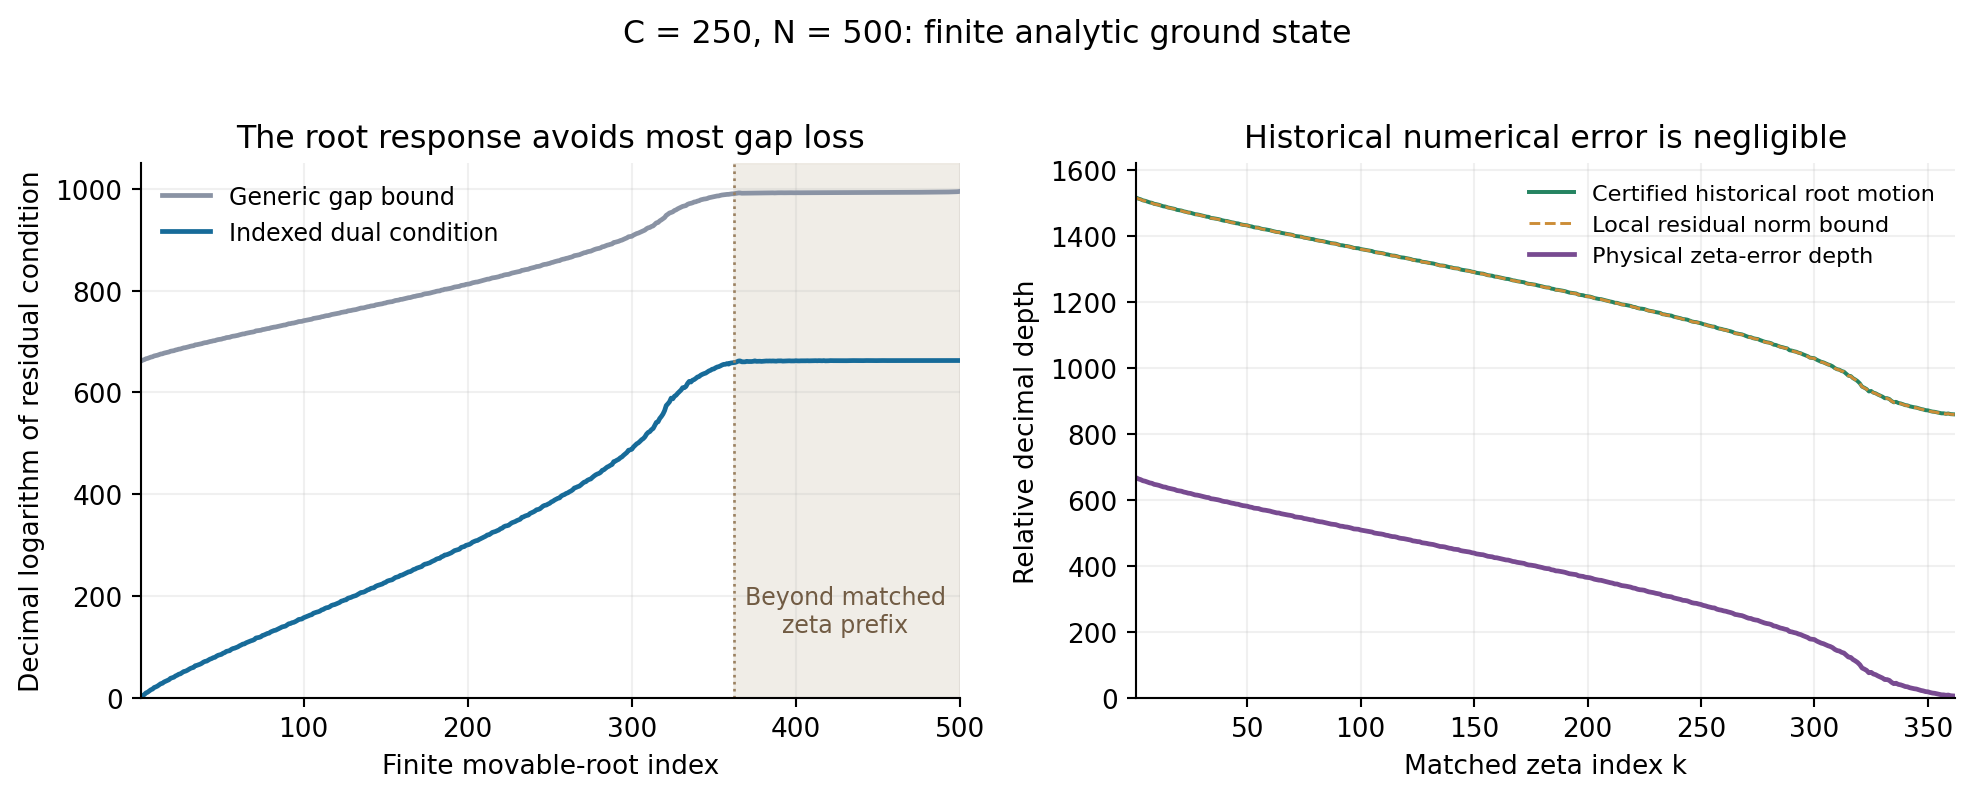
\includegraphics[width=\textwidth]{figures/indexed_dual_precision.png}
\caption{Finite indexed conditioning and historical source error at
$C=250,N=500$. Left: the root-specific dual avoids hundreds of decimal
digits of the generic gap penalty. Shading marks movable indices beyond
the 362-root matched zeta prefix. Right: the certified historical root
motion and the local residual norm estimate are far smaller than the
physical zeta error. Higher depth means smaller error.}
\label{fig:indexed-dual-precision}
\end{figure}
